\documentclass[11pt,a4paper,titlepage,oneside]{article}
\usepackage{LabProtocol}

\exercise{Exercise I}

% enter your data here
\authors{
	Cristian Avram, Matr. Nr. 01304470 \par
	{\small e01304470@student.tuwien.ac.at} \par
}
\date{}



\begin{document}

\maketitle

%%%%%%%%%%%%%%%%%%%%%%%%%%%%%%%%%%%%%%%%%%%%%%%%%%%%%%%%%%%%%%%%%%%%%%%%%%%%%%%%
%%%%%%%%%%%%%%%%%%%%%%%%%%%%%%%%%%%%%%%%%%%%%%%%%%%%%%%%%%%%%%%%%%%%%%%%%%%%%%%%
\Task{Structural modeling}
\begin{figure}[h!]
	\centering
	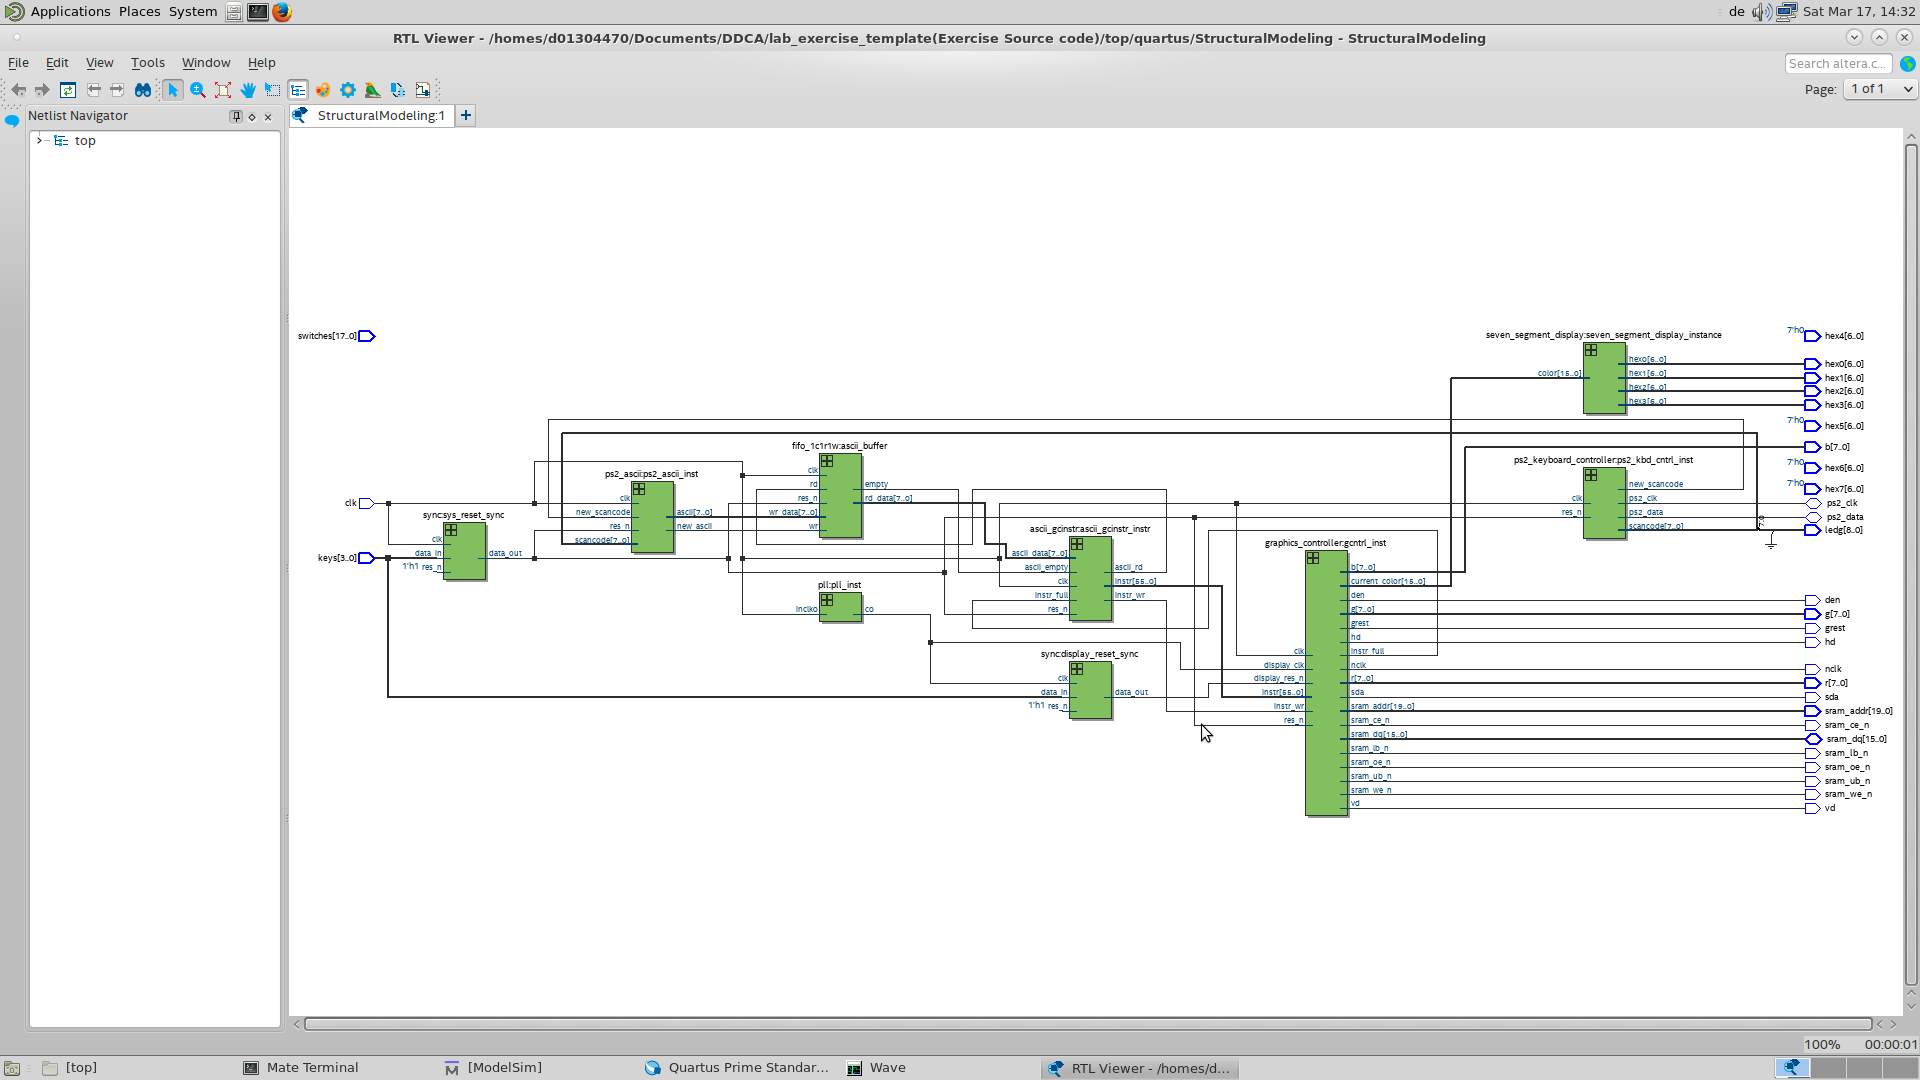
\includegraphics[width=1.0\linewidth]{task1 - RTL.png} % Use this command for your actual pictures
	\caption{Screenshot showing the top level design in the RTL netlist viewer}
\end{figure}



%%%%%%%%%%%%%%%%%%%%%%%%%%%%%%%%%%%%%%%%%%%%%%%%%%%%%%%%%%%%%%%%%%%%%%%%%%%%%%%%
%%%%%%%%%%%%%%%%%%%%%%%%%%%%%%%%%%%%%%%%%%%%%%%%%%%%%%%%%%%%%%%%%%%%%%%%%%%%%%%%
\Task{Seven Segment Display I}

\begin{qa}
	\question{Are the \textsf{hex*} signals high or low-active? Explain!}
	\answer{ The \textbf{hex*} signals are \textbf{low active}. This means, that when you want to see something on the seven segment display, you need to give them value 0 in order to have them active.}
\end{qa}

%%%%%%%%%%%%%%%%%%%%%%%%%%%%%%%%%%%%%%%%%%%%%%%%%%%%%%%%%%%%%%%%%%%%%%%%%%%%%%%%
%%%%%%%%%%%%%%%%%%%%%%%%%%%%%%%%%%%%%%%%%%%%%%%%%%%%%%%%%%%%%%%%%%%%%%%%%%%%%%%%
\Task{Behavioral Simulation}
\begin{figure}[h!]
	\centering
	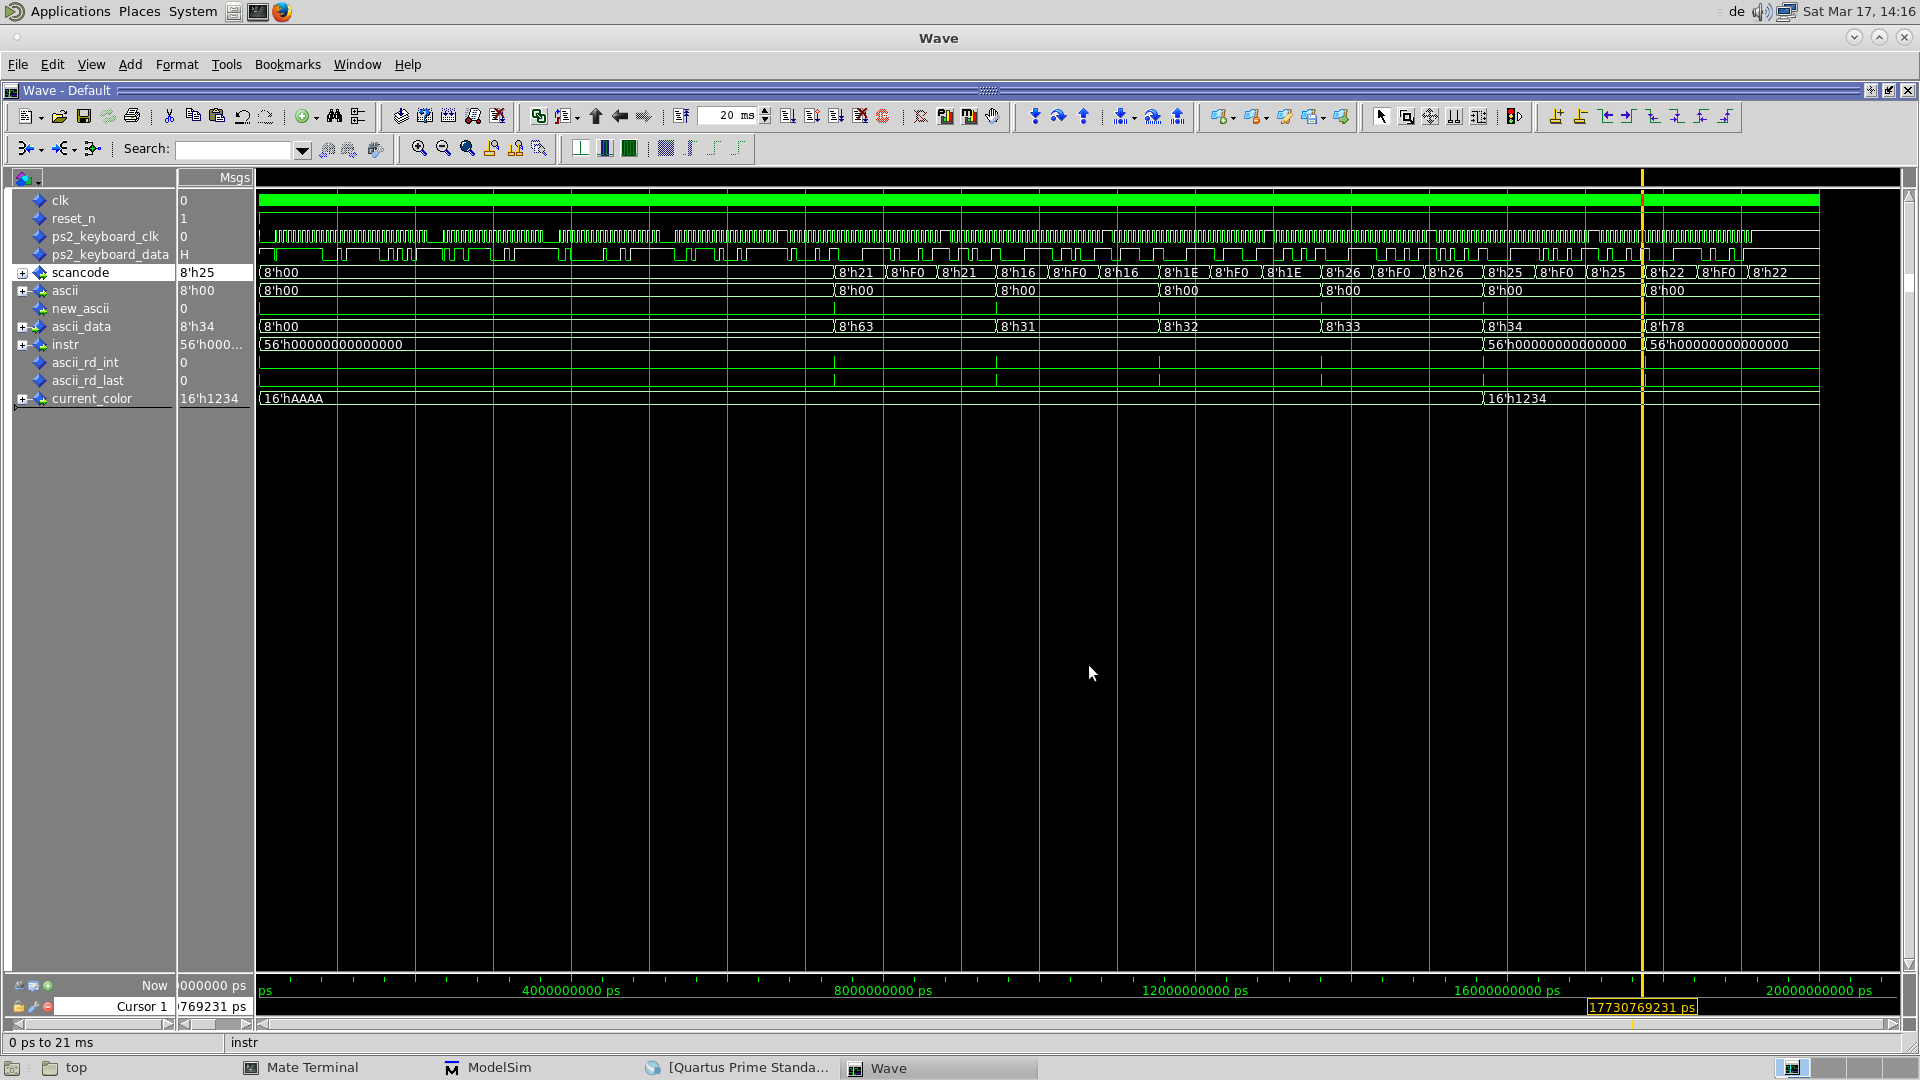
\includegraphics[width=1.0\linewidth]{task3 - 4 Propagation.png} % Use this command for your actual pictures
	\caption{Simulation showing the character propagation through the system}
\end{figure}


\begin{figure}[ht!]
	\centering
	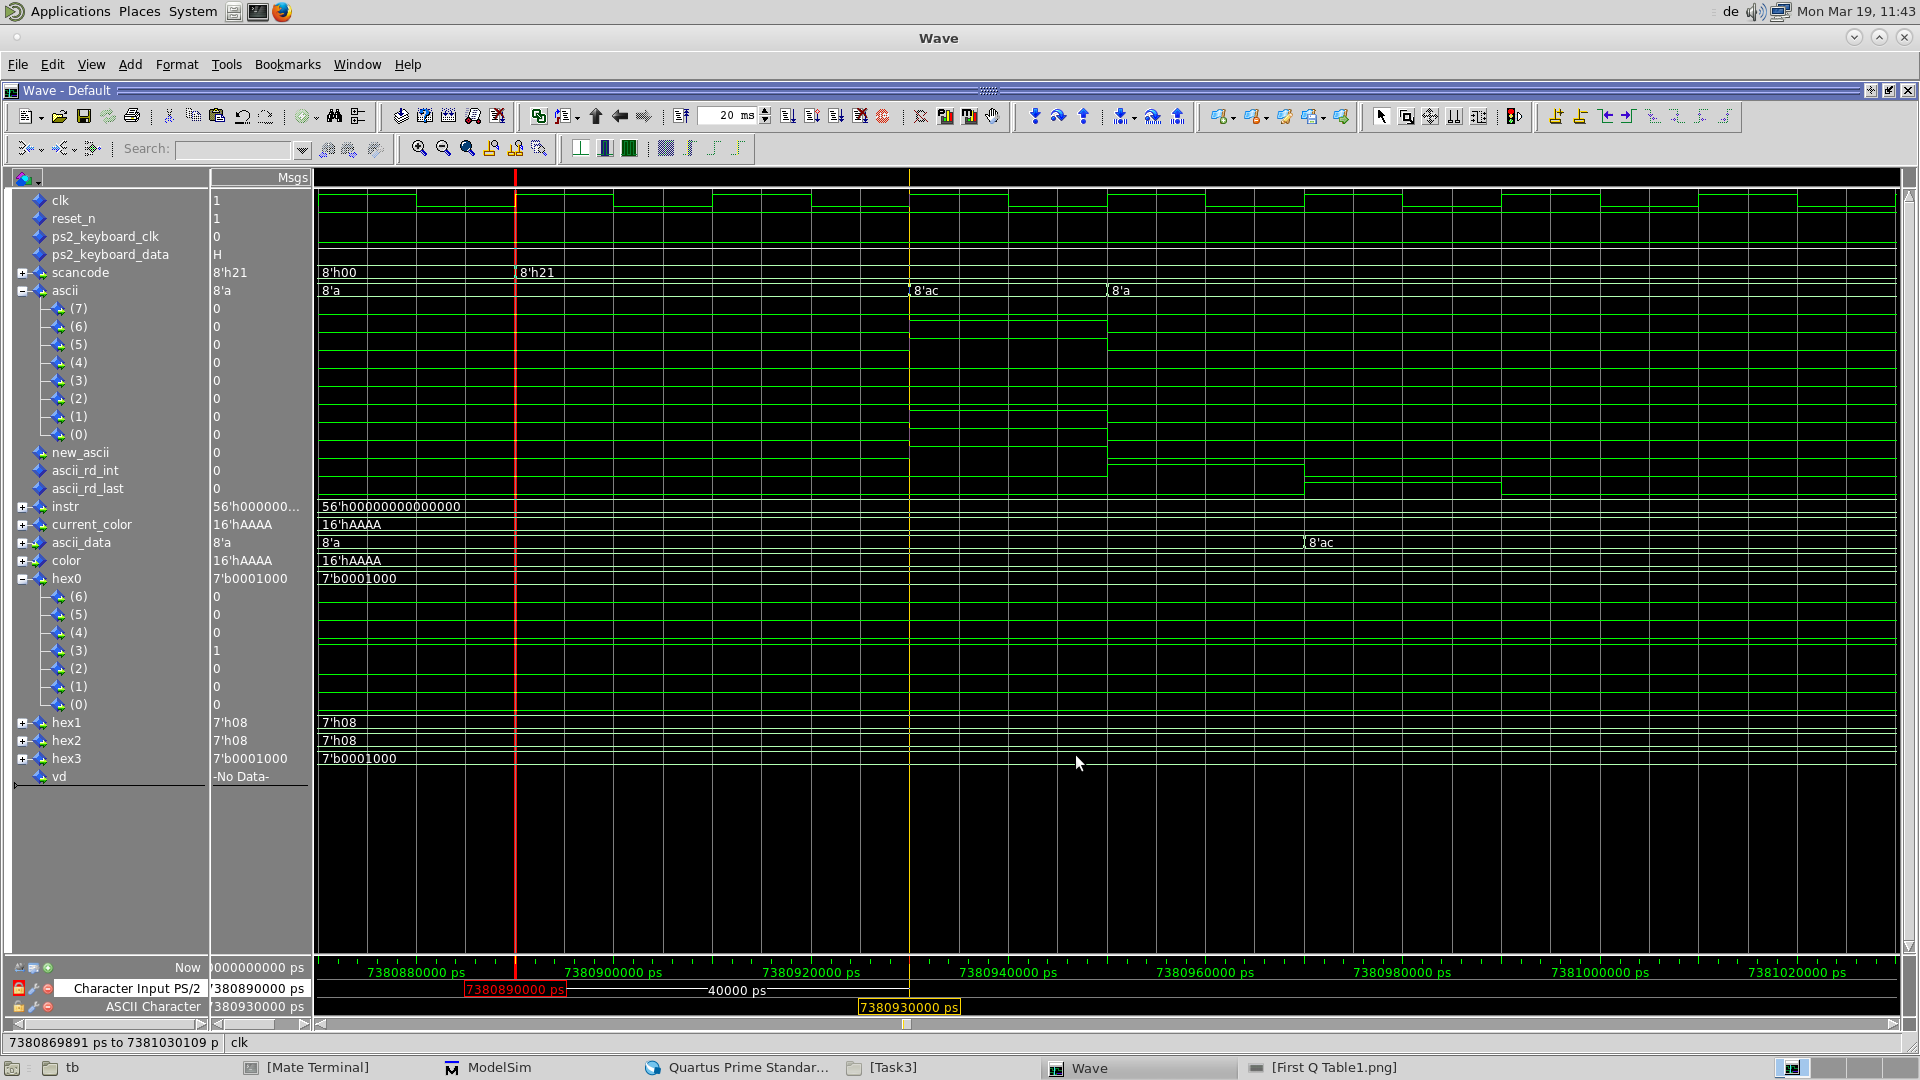
\includegraphics[width=1.0\linewidth]{FirstQ - Table1.png} 
	\caption{Interval Measurement using markers - Q1}
\end{figure}

\begin{figure}[ht!]
	\centering
	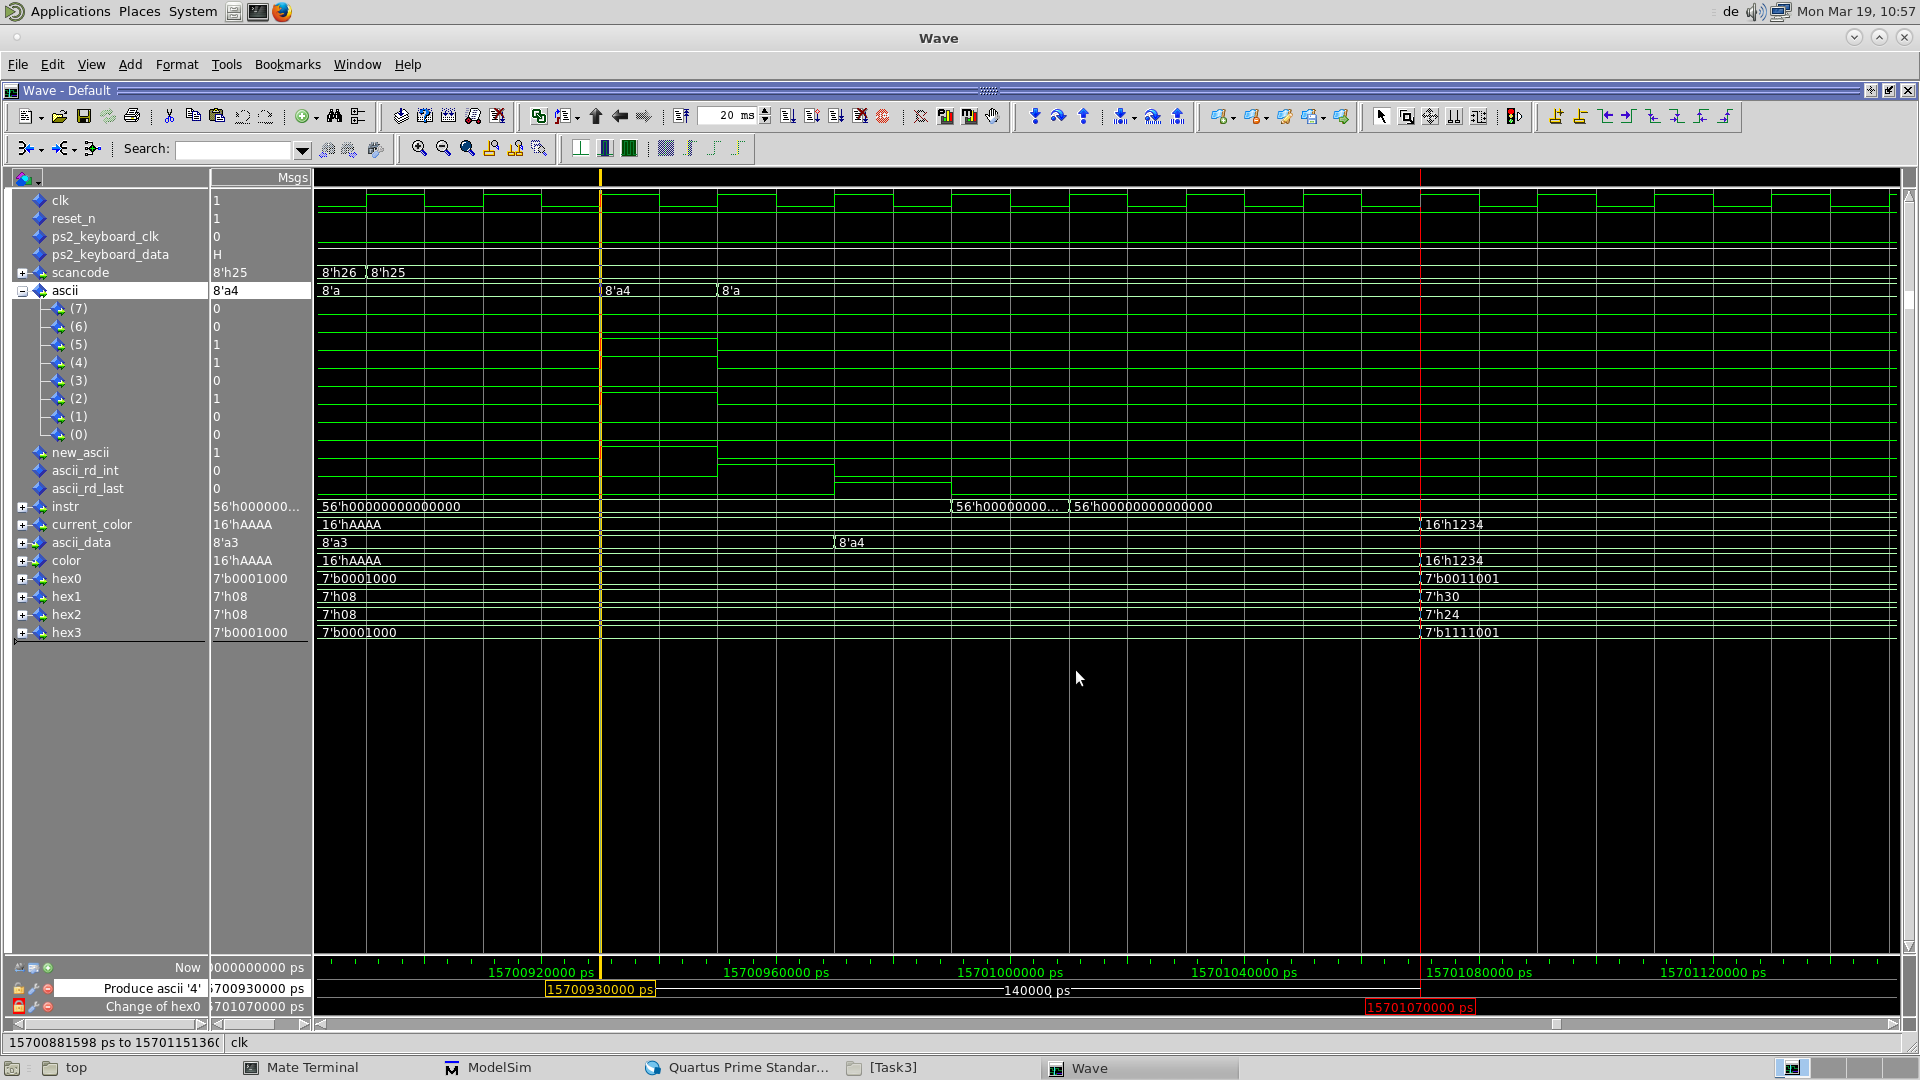
\includegraphics[width=1.0\linewidth]{SecondQ - Table1.png} 
	\caption{Interval Measurement using markers - Q2}
\end{figure}

\begin{figure}[ht!]
	\centering
	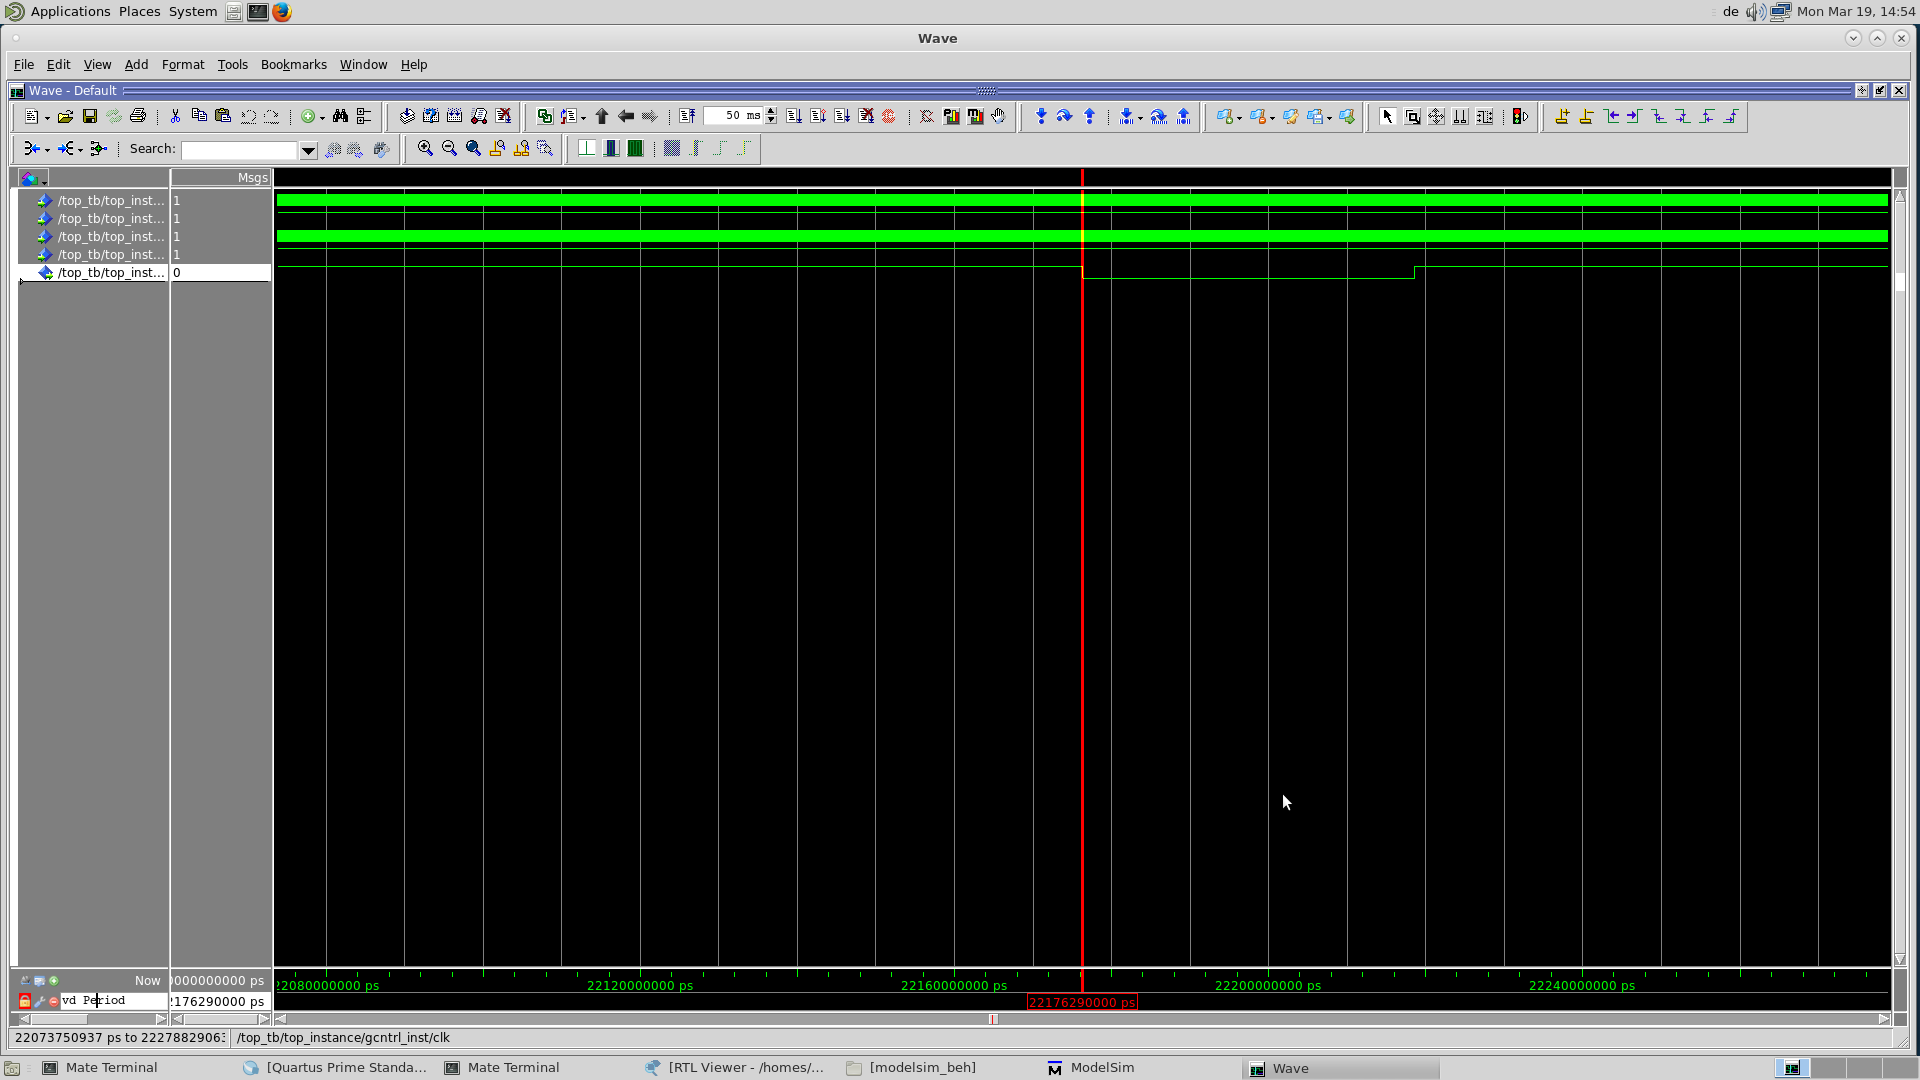
\includegraphics[width=1.0\linewidth]{ThirdQ - Table1.png} 
	\caption{Interval Measurement using markers - Q3}
\end{figure}

\begin{table}[ht!]
	\centering
	\caption{Timing measurements}
		\begin{tabular}{|p{0.8\textwidth}|l|}
		\hline
		Time                                                                 & Value  \\ \hline 
		First transition of a character input on the PS/2 interface to ASCII character output of \emph{ps2\_ascii} & 40 ns   \\
		Output of the last ASCII character ('4') to the seven segment display changing its output                       & 140 ns   \\
		1/Display frame rate (\textsf{vd} period)                        & 22,176 ms   \\ \hline
	\end{tabular}
\end{table}

%
% Information for the time period:
% First transition of a character input on the PS/2 interface to ASCII character output of \emph{ps2\_ascii}
% You may measure this interval for any of the characters input over the PS/2 interface.
% Just find the right PS/2 frame associated with the character you want to use for your measurement.
%

\begin{qa}
	\question{How long is the execution time of the clear screen command. How can you determine when the command has finished execution by just observing the signals to the SRAM?}
	\answer{The execution time is 45,79ms. It can be identified using $ top\_tb.vhd $ file by adding $ sram\_dq $ signal. The Length of the simulation should be around 80ms.}
\end{qa}


\begin{qa}
	\question{Describe how the bug in the \emph{ps2\_ascii} component affects the design.}
	\answer{The Bug being referred is the one in $ ps2\_ascii.vhd $ and it consists of "Y" and "y" being mapped to letter "Z" and "z". By using the command $ make \  sim\_fileio $ we are greeted with and Error that says "y" expected=0x79, actual=0x7a, and "Y" expected=0x59, actual=0x5a. The only thing to do is to change the values in the above mentioned document and redo the test.  }
\end{qa}

%%%%%%%%%%%%%%%%%%%%%%%%%%%%%%%%%%%%%%%%%%%%%%%%%%%%%%%%%%%%%%%%%%%%%%%%%%%%%%%%
%%%%%%%%%%%%%%%%%%%%%%%%%%%%%%%%%%%%%%%%%%%%%%%%%%%%%%%%%%%%%%%%%%%%%%%%%%%%%%%%
\Task{Postlayout Simulation}
\begin{qa}
	\question{Different propagation delays: How long is the transition time you measured when the seven segment display output bus changes its value and multiple signals toggle?}
	\answer{Based on $ StructuralModeling\_7\_1200mv\_Oc\_slow.vho $ file \newline and $ StructuralModeling\_7\_1200mv\_Oc\_vhd\_slow.sdo $ } the transition time is  3572 ps.
\end{qa}

\begin{figure}[ht!]
	\centering
    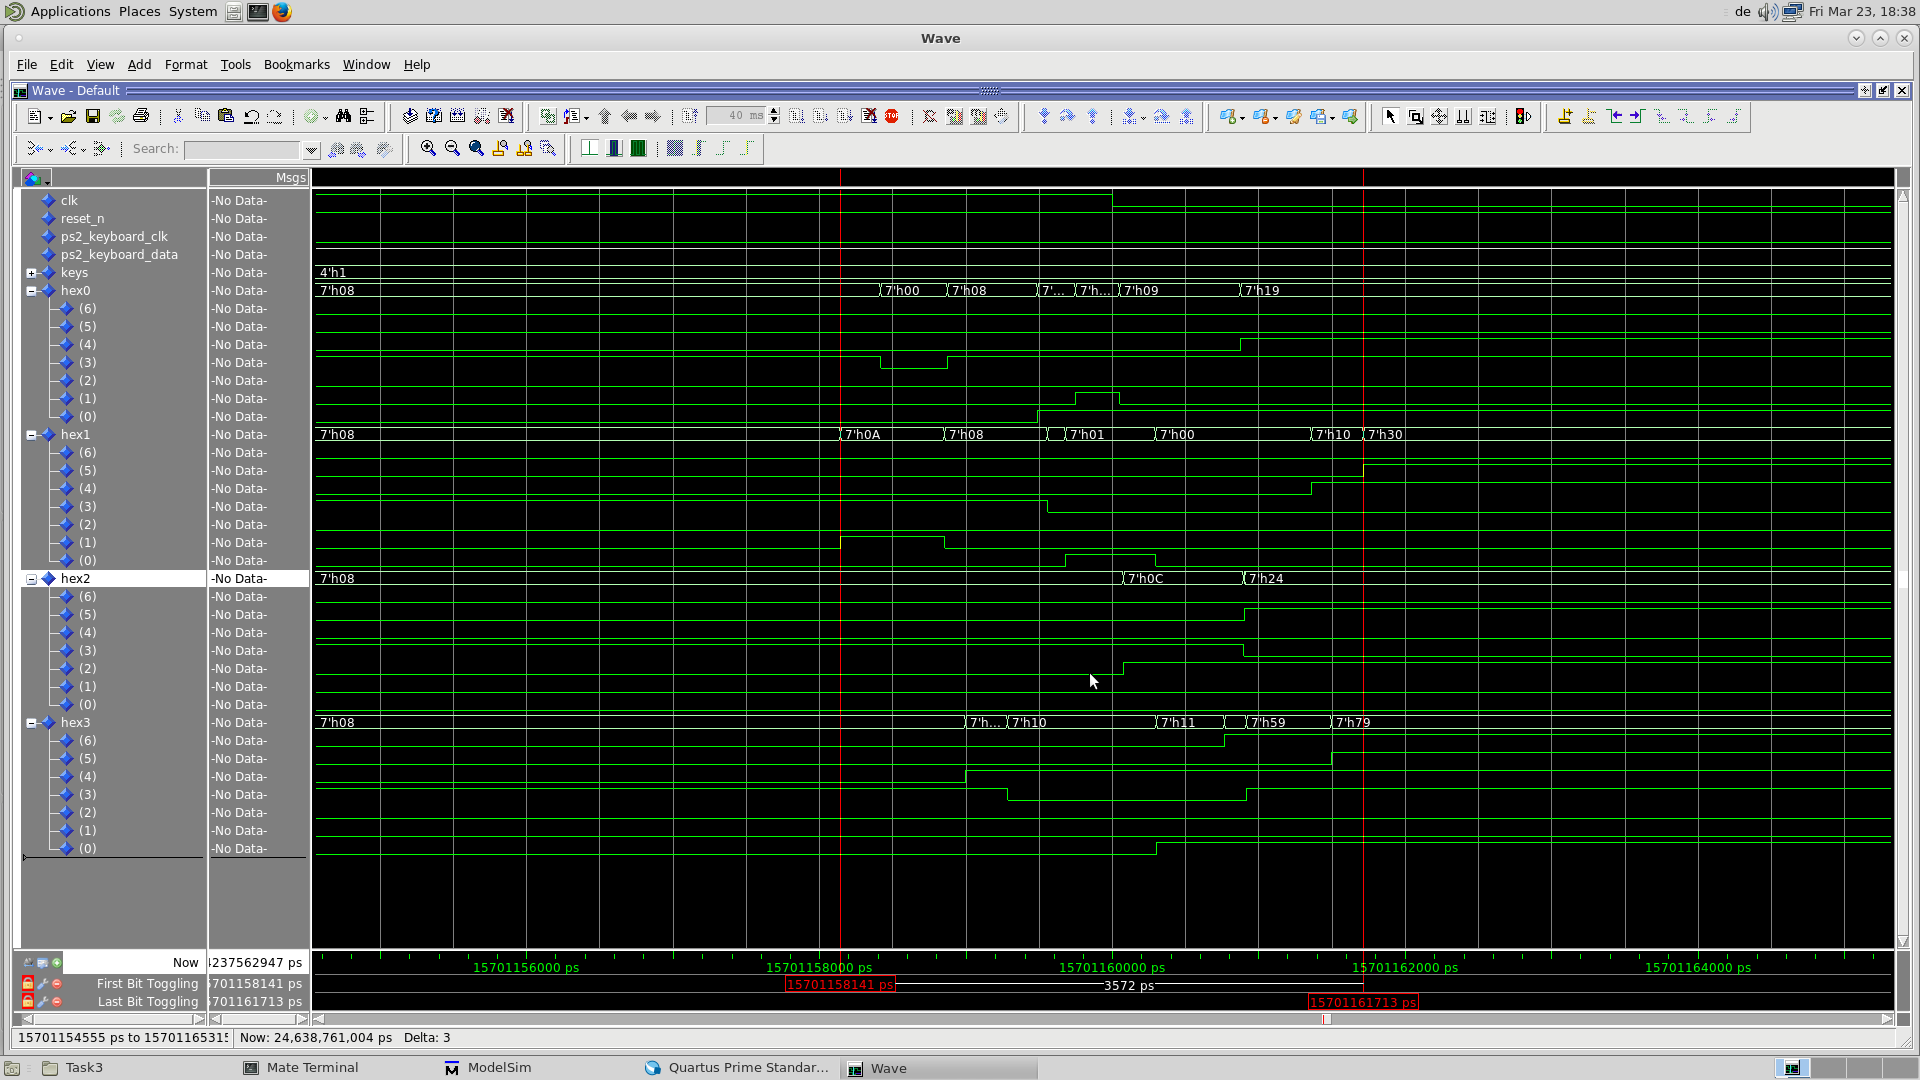
\includegraphics[width=1.0\linewidth]{task4.png}
	\caption{Different propagation delays on the seven segment display bus}
\end{figure}

%%%%%%%%%%%%%%%%%%%%%%%%%%%%%%%%%%%%%%%%%%%%%%%%%%%%%%%%%%%%%%%%%%%%%%%%%%%%%%%%
%%%%%%%%%%%%%%%%%%%%%%%%%%%%%%%%%%%%%%%%%%%%%%%%%%%%%%%%%%%%%%%%%%%%%%%%%%%%%%%%
\Task{Seven Segment Display II}

\begin{figure}[h!]
	\centering
	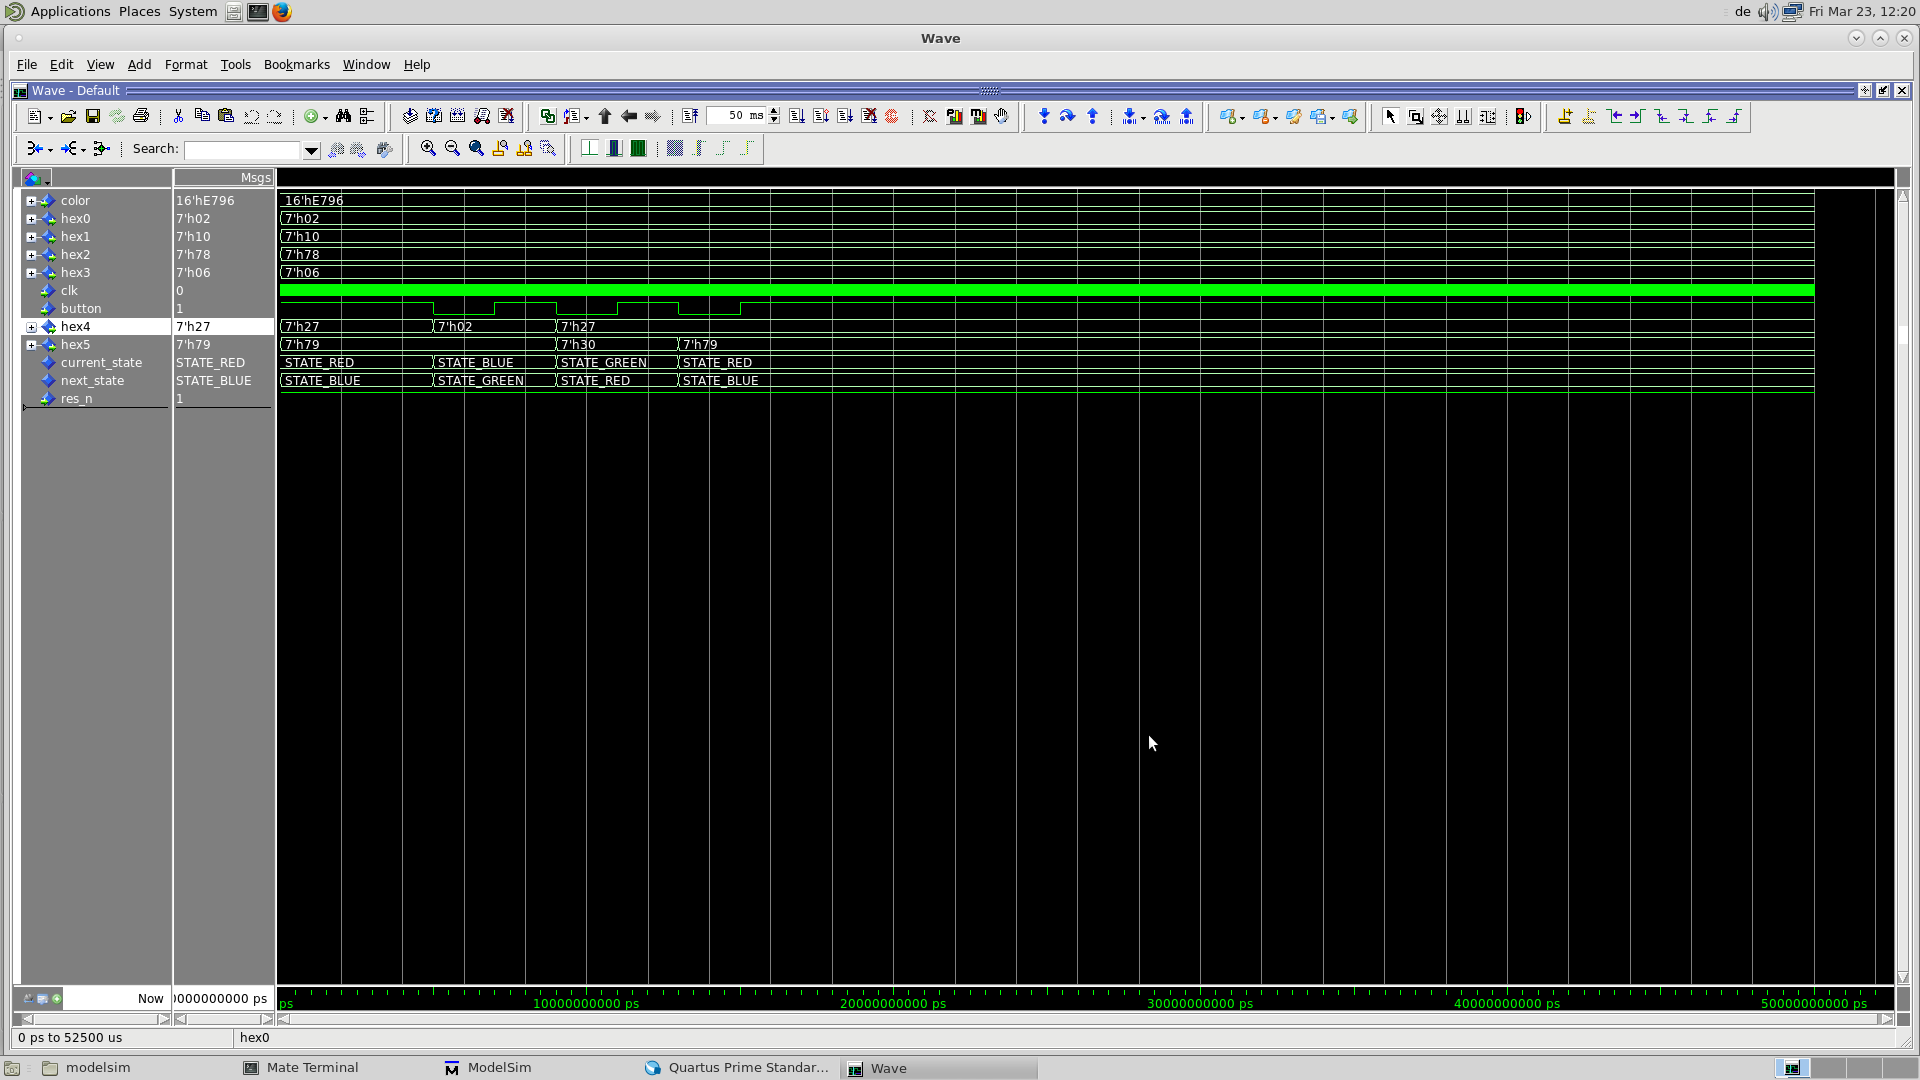
\includegraphics[width=1.0\linewidth]{task5 - decimal.png}
	\caption{Simulation of the extended seven segment display (3 button presses)}
\end{figure}

\begin{qa}
	\question{Argue why the output on the signals \textsf{hex\{4-5\}} is correct.}
	\answer{The RGB color signal will have $ hE795 $ value. It will consist of $ h1c $ as red channel, $ h15 $ as blue channel, and $ h3c $ as green channel }
\end{qa}

%%%%%%%%%%%%%%%%%%%%%%%%%%%%%%%%%%%%%%%%%%%%%%%%%%%%%%%%%%%%%%%%%%%%%%%%%%%%%%%%
%%%%%%%%%%%%%%%%%%%%%%%%%%%%%%%%%%%%%%%%%%%%%%%%%%%%%%%%%%%%%%%%%%%%%%%%%%%%%%%%
\Task{Serial Port}
\begin{figure}[ht!]
	\centering
	%%%%%%%%%%%%%%%%%%%%%%%% 
	% Include markers for measuring the duration of the frame (including the start-bit).
	%%%%%%%%%%%%%%%%%%%%%%%% 
	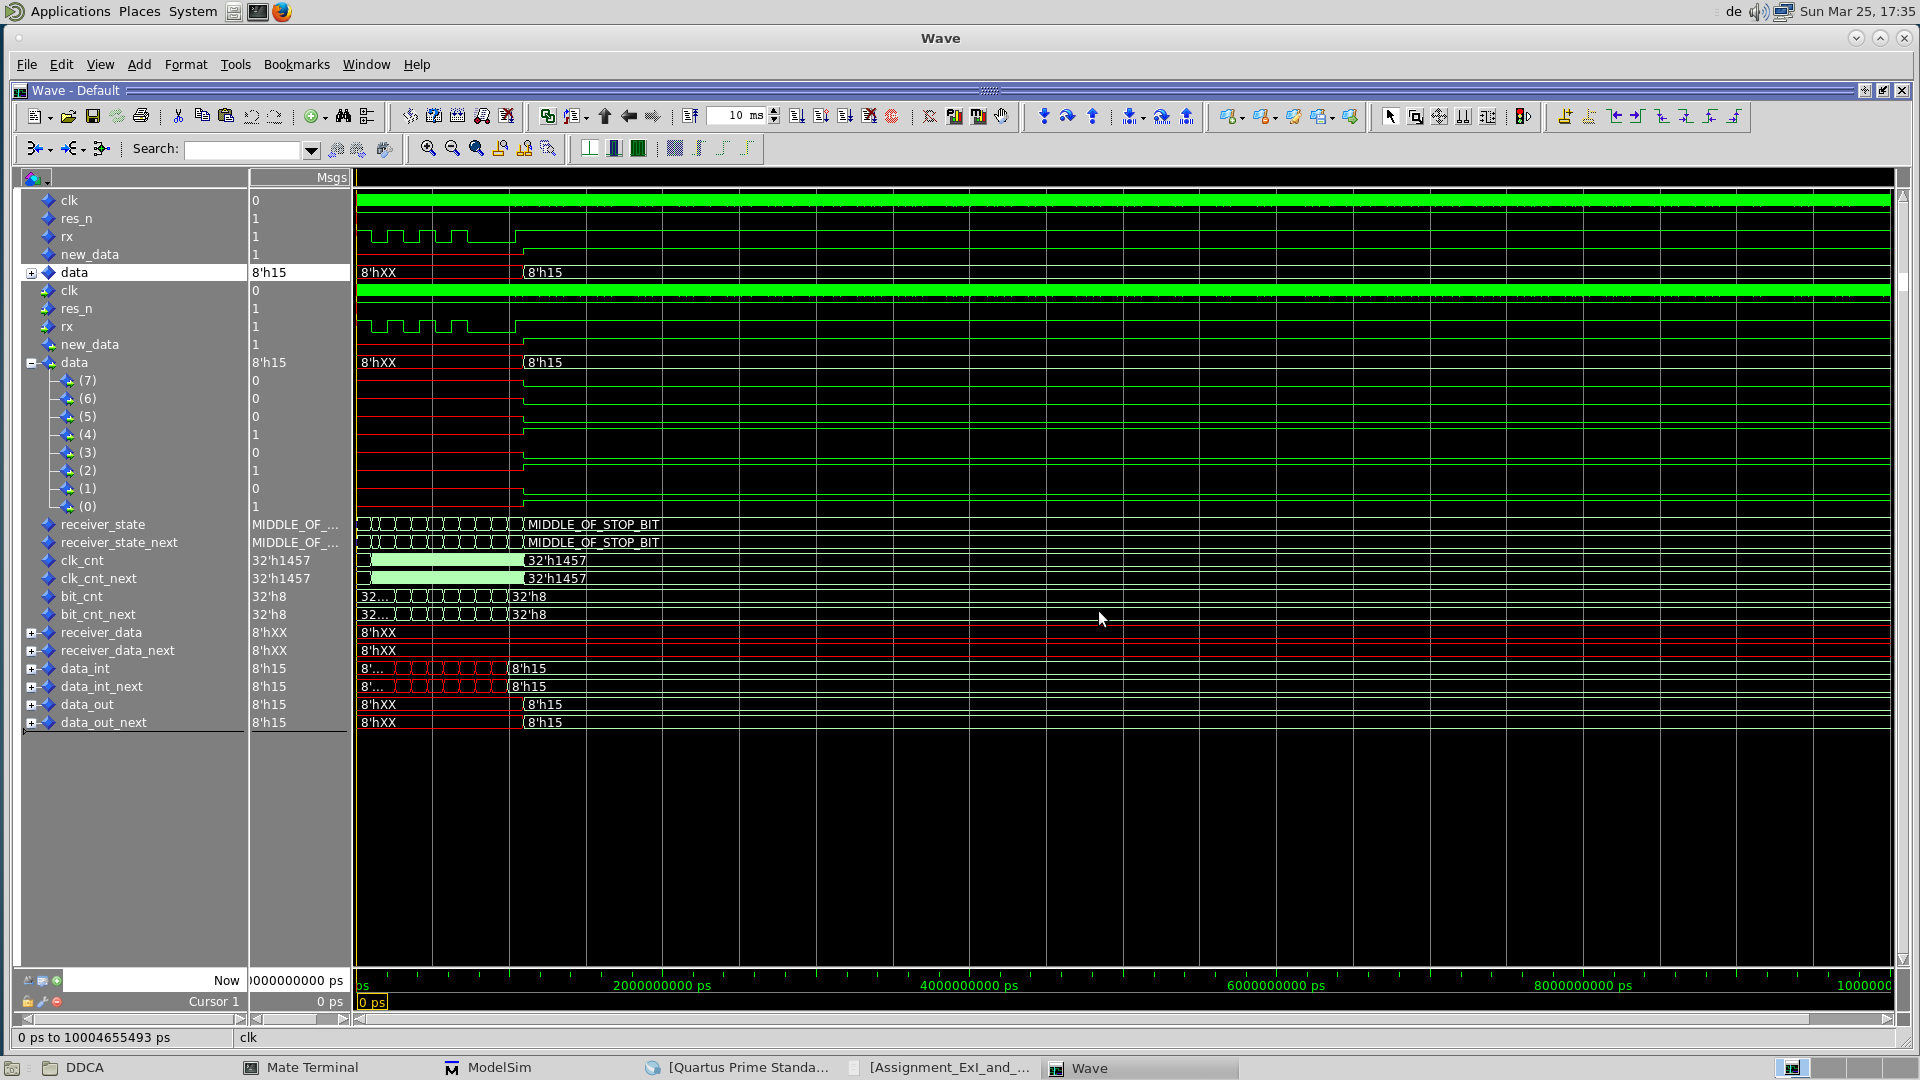
\includegraphics[width=1.0\linewidth]{task6 - Simulation receiver.png}
	\caption{Screenshot of a simulation showing the reception of a whole UART frame.}
\end{figure}

\begin{qa}
	\question{Which baudrate did you use for the above simulation? How long should the transmission take for the whole frame (including start and stop bit)? What is the time you measured in the simulation (not including the stop bit)?}
	\answer{I used 9600 bps as Baudrate value, which means that 1 bit will be transferred in 1/9600 seconds. In total, we have 10 bits including start, stop and data bits. The time that I measured is 941$ \mu s $.}
\end{qa}


\begin{qa}
	\question{Why does the state machine only count to \emph{CLK\_DIVISOR-2} and not \emph{CLK\_DIVISOR-1}?}
	\answer{It does need to go back to $ WAIT\_DATA\_BIT $, so this is why it reserves one last clock cycle for that. For every clock cycle, it moves to another state.}
\end{qa}

\begin{qa}
	\question{What is the purpose of the \emph{MIDDLE\_OF\_START\_BIT} state of the receiver FSM? Is it really necessary or could it be optimized away?}
	\answer{The purpose is to prevent glitches as start bit. Another reason, is to make sure that the middle of start bit is still low.}
\end{qa}


\begin{table}[h!]
	\centering
	\caption{Resouce usage of the serial module (including all submodules).}
	\begin{tabular}{|l|l|l|l|}
	\hline
	& LC Combinationals & LC Registers & Memory      \\ \hline 
	Absolute number      &              302     &           236   &         0    \\
	\% of whole design   &               1374    &         1618    &        56320   \\
	\% of whole FPGA resources &           3        &       1        &     1         \\ \hline
	\end{tabular}
\end{table}

%%%%%%%%%%%%%%%%%%%%%%%%%%%%%%%%%%%%%%%%%%%%%%%%%%%%%%%%%%%%%%%%%%%%%%%%%%%%%%%%
%%%%%%%%%%%%%%%%%%%%%%%%%%%%%%%%%%%%%%%%%%%%%%%%%%%%%%%%%%%%%%%%%%%%%%%%%%%%%%%%



%\clearpage
%\section*{Feedback \& Comments}
%\input{feedback}

\end{document}
